% !TeX spellcheck = cs_CZ
%{\tikzset{external/prefix={tikz/FYZI/}}
% \tikzset{external/figure name/.add={ch38_}{}}
%=========================== Kapitola: Souvislost mezi vlnovým a korpuskulárním hlediskem =========
\setchaptertoc
\chapter{Souvislost mezi vlnovým a korpuskulárním hlediskem}\label{fyz:IchapXXXVIII}
  \section{Amplitudy vln pravděpodobnosti}\label{fyz:IchapXXXVIIIsecI}
    V této kapitole se zamyslíme nad vztahem mezi vlnovým a korpuskulárním hlediskem. Z poslední
    kapitoly už víme, že ani vlnové, ani korpuskulární hledisko není správné. Obvykle jsme se
    snažili vše podávat přesně nebo alespoň tak přesně, že se to nemuselo měnit, když se naše
    vědomosti dostaly dále - mohli jsme je rozšířit, ale nikdy jsme je nemuseli měnit! Pokusíme-li
    se mluvit o vlnovém nebo korpuskulárním obraze, oba jsou přibližné a oba se budou muset změnit.
    Proto ani to, co se v této kapitole dozvíme, nebude v určitém smyslu přesné; bude to
    polointuitivní argumentace, která se později upřesní, ale některé věci se změní, budeme-li je
    interpretovat kvantově - mechanicky správně. Důvod, proč to tak uděláme, je ten, že se nehodláme
    zabývat přímo kvantovou mechanikou, ale chceme získat aspoň určitou představu o jevech, s nimiž
    se setkáme. Navíc, protože se všechny naše zkušenosti týkají vln a částic, abychom pochopili, oč
    tu jde, dřív než zvládneme celou matematiku kvantově -mechanických amplitud, je velmi výhodné
    použít vlnové a korpuskulární představy. Přitom se budeme snažit ilustrovat nejslabší místa, ale
    většinou budeme téměř zcela korektní - je to zcela věc interpretace.

    Především víme, že nový způsob reprezentace světa v kvantové mechanice - nový rámec - spočívá v
    tom, že každé možné události přísluší amplituda. Týká-li se událost dopadu jedné částice, můžeme
    určit amplitudu pravděpodobnosti, že se částice najde v různých časech na různých místech.
    Pravděpodobnost nalezení částice je pak úměrná druhé mocnině absolutní hodnoty amplitudy. Obecně
    se amplituda pravděpodobnosti, že najdeme částici na různých místech v různých časech, mění s
    polohou a časem. 

    Ve zvláštním případě se amplituda mění v prostoru a čase sinusoidálně jako \(e^{\imath(\omega
    t−\vr{k}\cdot\vr{r})}\) (nezapomínejme, že tyto amplitudy jsou komplexní a ne reálné) a
    zahrnuje určitou frekvenci \(\omega\) vlnový vektor \(\vr{k}\). Ukazuje se, že v klasické
    limitě to odpovídá situaci, kde jsme si představovali, že máme částici se známou energií \(E\),
    jež souvisí s frekvencí vztahem
    \begin{equation}\label{fyz:eq598}
      E = \hbar\omega        % E=ℏω,
    \end{equation}
    a známou hybností \(\vect{p}\), která souvisí s vlnovým vektorem vztahem
    \begin{equation}\label{fyz:eq599}
      \vr{p} = \hbar\vr{k}    % p=ℏk
    \end{equation}

    \begin{figure}[ht!] %\ref{fyz:fig432}
      \centering
      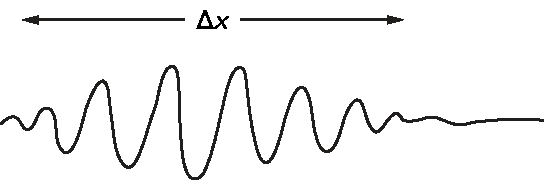
\includegraphics[width=0.8\linewidth]{fyz_fig432.pdf}
      \caption{Vlnový balík délky \(\Delta x\) (\cite[s.~510]{Feynman01})}
      \label{fyz:fig432}
    \end{figure}

    To znamená, že představa částice je omezená. Představa částice - její polohy, hybností atd. -
    kterou tak často používáme, je určitým způsobem neuspokojivá. Například, je-li amplituda
    pravděpodobnosti toho, že najdeme částici na různých místech, dána funkcí \(e^{\imath(\omega
    t−\vr{k}\cdot\vr{r})}\), jejíž druhá mocnina absolutní hodnoty je konstantní, bude to znamenat,
    že pravděpodobnost nalezení částice je pro všechny body stejná. Pak nevíme, kde se částice
    nachází; částice může být kdekoliv a její poloha je velmi neurčitá.
    
    Na druhé straně, je-li poloha částice více méně dobře známá a umíme ji předpovědět dost přesně,
    pravděpodobnost toho, že se najde na různých místech, musí být omezena na oblast délky \(\Delta
    x\). Mimo tuto oblast je pravděpodobnost nulová. Tato pravděpodobnost je rovna druhé mocnině
    absolutní hodnoty amplitudy, proto, je-li druhá mocnina absolutní hodnoty rovna nule, bude rovna
    nule i amplituda. Dostáváme vlnový impulz o délce \(\Delta x\) (obr. \ref{fyz:fig432}) a jeho
    vlnová délka (vzdálenost mezi nulovými hodnotami) je to, co odpovídá hybnosti částice.

    Zde se setkáváme s podivnou vlastností vln. Je to velmi snadná věc, která nijak nesouvisí s
    kvantovou mechanikou. Něco, co zná každý, kdo se zabývá vlněním, i když nezná kvantovou
    mechaniku: \emph{Pro krátký vlnový impulz nemůžeme jednoznačně definovat vlnovou délku}. Vlnové
    číslo je neurčité, souvisí s konečnou délkou impulzu, a proto je neurčitá i hybnost částice.

  \section{Měření polohy a hybnosti}\label{fyz:IchapXXXVIIIsecII}
    Podívejme se na dva příklady, abychom si ozřejmili, proč musí podle kvantové mechaniky existovat
    neurčitost v poloze nebo v hybnosti. Už dříve jsme viděli, že kdyby něco takového neexistovalo -
    kdyby bylo možné současně měřit polohu i hybnost - byl by to paradox. To naštěstí nenastává a
    skutečnost, že taková neurčitost vyplývá z vlnového obrazu svědčí o tom, že vše je vzájemně
    konzistentní.

    \begin{figure}[ht!] %\ref{fyz:fig433}
      \centering
      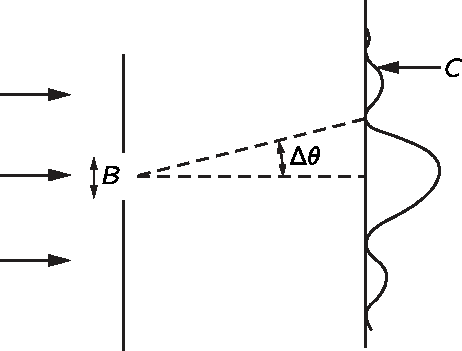
\includegraphics[width=0.8\linewidth]{fyz_fig433.pdf}
      \caption{Difrakce částic procházejících štěrbinou (\cite[s.~511]{Feynman01})}
      \label{fyz:fig433}
    \end{figure}

    Uvedeme příklad, na němž lze snadno pochopit, jaký je vztah mezi polohou a hybností.
    Předpokládejme, že máme štěrbinu a částice s určitou energií, jež přilétají velmi zdaleka, takže
    v podstatě všechny letí vodorovně (obr. 38.2). Budeme se zajímat o svislou složku hybnosti.
    Všechny částice mají, v klasickém smyslu, určitou horizontální hybnost \(p_0\), takže, v
    klasickém smyslu, známe vertikální hybnost \(p_y\) každé částice předtím, než proletí štěrbinou.
    Částice neletí ani směrem vzhůru, ani dolů, neboť přilétá od velmi vzdáleného zdroje -a proto je
    její vertikální hybnost rovna nule. Předpokládejme, že dále letí částice štěrbinou vertikální
    šířky \(B\). Po průletu štěrbinou známe vertikální polohu - souřadnici \(y\) a to s pozoruhodnou
    přesností \(\pm B\). Neurčitost polohy \(\Delta y\) je tedy rovna řádově \(B\). Mohlo by se
    zdát, vzhledem k tomu, že hybnost částice má čistě horizontální směr, bude \(\Delta p_y\) rovno
    nule, ale není tomu tak. Věděli jsme, že hybnost je horizontální, ale už to nevíme. Dříve, než
    částice proletěly otvorem, neznali jsme jejich vertikální polohy a nyní, tím, že jsme je nechali
    proletět otvorem, jsme ztratili informaci o jejich vertikální hybnosti! Proč? Podle vlnové
    teorie při průchodu vln štěrbinou dochází k jejich rozmazání nebo difrakci, podobně jako u
    světla. Proto existuje určitá pravděpodobnost, že částice nevyletují ze štěrbiny úplně přímo.
    Difrakční efekt rozmaže obraz jejich rozmístění a úhel, který můžeme definovat jako úhel prvního
    minima, je mírou neurčitosti konečného úhlu.

    Jak dochází k rozmazání obrazu? Řekneme-li, že je rozmazaný, znamená to, že existuje určitá
    pravděpodobnost, že částice se vychýlí nahoru nebo dolů, tj. že bude mít složku hybnosti ve
    směru nahoru nebo dolů. Mluvíme o pravděpodobnosti a o částici, protože difrakční obraz můžeme
    proměnit pomocí počítače částic, který, když zachytí částici, dejme tomu v bodě C na obr.
    \ref{fyz:fig433}, zachytí celou částici, takže v klasickém smyslu, aby se částice dostala od
    štěrbiny do C, musí mít nějakou vertikální hybnost.

    Abychom dostali aspoň přibližnou představu o rozmazání hybnosti \(p_y\), uvědomme si, že
    rozmazání vertikální hybnosti je rovno \(p_0Δθ\), kde \(p_0\) je horizontální hybnost. Jak velké
    je \(\Delta \Theta\) v difrakčním obraze? Víme, že první minimum nastává při takovém úhlu
    \(Δθ\), při němž je dráha vln od jednoho okraje štěrbiny delší o vlnovou délku než dráha vln od
    druhého okraje štěrbiny - zdůvodnili jsme si to už dříve (v kapitole 30). Proto Δθ je λ/B, takže
    \(Δp_y\) je v tomto experimentu \(p_0λ/B\). Vidíme, že čím víc zmenšíme \(B\) a přesněji určíme
    polohu, tím bude difrakční obraz širší. Vzpomeňme si, že čím víc jsme uzavřeli štěrbinu v našem
    experimentu s mikrovlnami, tím větší byla intenzita ve vzdálených polohách. Takže, čím užší bude
    štěrbina, tím víc se celý obraz roztáhne a tím je větší pravděpodobnost, že naměříme příčnou
    složku hybnosti částice. Neurčitost vertikální hybnosti je tedy nepřímo úměrná neurčitosti
    \(y\). Vidíme, že jejich součin je roven p0λ. Ale λ je vlnová délka, \(p_0\) je hybnost a podle
    kvantové mechaniky součin vlnové délky a hybnosti dává Planckovu konstantu \(h\). Dostali jsme
    tak pravidlo, že součin neurčitosti vertikální hybnosti a neurčitosti vertikální polohy je
    řádově roven \(h\):
    \begin{equation}\label{fyz:eq597}
      \boxed{ΔyΔp_y ≥ \hbar/2}
    \end{equation}
    Nemůžeme sestrojit zařízení, jež by umožnilo ze známé vertikální polohy částice předpovědět i
    její vertikální pohyb s větší přesností, než je dána pomocí (\ref{fyz:eq597}). Neurčitost
    vertikální hybnosti musí být větší než \(\hbar/2Δy\), kde \(Δy\) je neurčitost, s níž známe
    polohu.

    Lidé občas říkají, že celá kvantová mechanika je pochybená. Když částice přilétávala zleva, měla
    nulovou vertikální hybnost a nyní, když prošla štěrbinou a dopadla na detektor, je její poloha
    známa. Zdá se, že jak poloha, tak i hybnost jsou známé s libovolnou přesností je to tak, po
    dopadu částice můžeme určit její polohu a hybnost, kterou musela mít, aby dopadla na dané místo.
    Je to pravda, ale netýká se to relace neurčitosti (\ref{fyz:eq597}). Rovnice (\ref{fyz:eq597})
    se vztahuje k možnosti předpovědět situaci na základě znalostí z minulosti. Co máme z toho, když
    řekneme: „Věděl jsem, jaká byla hybnost před průchodem štěrbinou a nyní znám polohu", když teď
    nevím nic o hybnosti. Skutečnost, že částice proletěla štěrbinou, nám nedovoluje předpovědět
    její vertikální hybnost. Mluvíme o prediktivní teorii, nejen o měřeních z minulosti. Musíme
    mluvit o tom, co dokážeme předpovědět.

    \begin{figure}[ht!] %\ref{fyz:fig434}
      \centering
      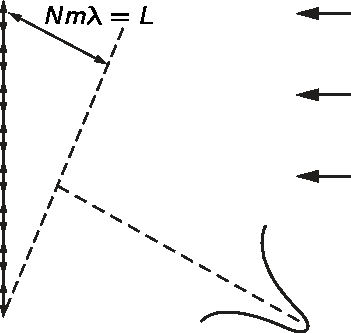
\includegraphics[width=0.7\linewidth]{fyz_fig434.pdf}
      \caption{Určení hybnosti pomocí difrakční mřížky (\cite[s.~513]{Feynman01})}
      \label{fyz:fig434}
    \end{figure}

    Nyní pojďme na celou věc z opačného konce. Proveďme si podrobnější kvantitativní analýzu dalšího
    příkladu téhož jevu. V předcházejícím příkladě jsme měřili hybnost klasickou metodou - uvažovali
    jsme o směru, rychlosti, úhlech atd., takže hybnost jsme určovali klasicky. Ale protože hybnost
    souvisí s vlnovým číslem, existuje další možnost, jak změřit hybnost částice (fotonu nebo
    podobně), jež nemá klasický analog, neboť je založena na rovnici (\ref{fyz:eq599}). Spočívá v
    měření vlnové délky. Pokusme se hybnost změřit tímto způsobem.
    
    Předpokládejme, že máme difrakční mřížku s velkým počtem vrypů (obr. \ref{fyz:fig434}) a že na
    ni nasměrujeme svazek částic. O tomto problému jsme mluvili často. Mají-li částice určitou
    hybnost, v určitém směru dostáváme, díky interferenci, ostré maximum. Mluvili jsme i o tom, jak
    přesně umíme určit hybnost, tj. jaká je rozlišovací schopnost této mřížky. Místo toho, abychom
    to znovu odvozovali, můžeme se odvolat na kapitolu \ref {fyz:IchapXXX}, kde vidíme, že relativní
    neurčitost při měření vlnové délky pomocí dané mřížky je \(1/Nm\), kde \(N\) je počet vrypů na
    mřížce a \(m\) je řád na difrakčním obraze. Takže
    \begin{equation}\label{fyz:eq600}
      \frac{Δλ}{λ}=\frac{1}{Nm}.
    \end{equation}
    Vztah (\ref{fyz:eq600}) lze napsat jako
    \begin{equation}\label{fyz:eq601}
      \frac{Δλ}{λ^2} = \frac{1}{Nmλ} = \frac{1}{L},
    \end{equation} 
    kde \(L\) je vzdálenost znázorněná na obr. \ref{fyz:fig434}. Je to rozdíl vzdáleností, jež musí
    projít vlna nebo cokoliv, když se odrazí od horního okraje mřížky a když se odrazí od dolního
    okraje. Vlny, které vytvářejí difrakční obraz, přicházejí od různých částí mřížky. První přiletí
    ta, která přichází od dolního okraje mřížky ze začátku vlnového signálu, další pocházejí od
    pozdějších částí vlnového signálu a odrážejí se od různých částí mřížky, až nakonec přiletí
    poslední, jež odpovídá bodu vzdálenému ve vlnovém signálu o vzdálenosti \(L\) od začátku. Proto,
    abychom dostali v našem spektru ostrou čáru, jež odpovídá pevné dané hybnosti s neurčitostí
    podle (\ref{fyz:eq600}) , musíme mít vlnový balík aspoň o délce \(L\) je-li balík kratší,
    nevyužijeme celou mřížku. Vlny vytvářející spektrum se odrážejí od velmi malé části mřížky a
    mřížka nepracuje, jak by měla – dostaneme velké úhlové rozložení. Aby bylo rozložení užší,
    musíme použít celou mřížku, aby se aspoň v některém okamžiku odrážel celý vlnový balík současně
    od různých částí mřížky. Proto, chceme-li, aby neurčitost vlnové délky byla menší, než udává
    vztah (\ref{fyz:eq601}), délka balíku musí být \(L\) Platí   
    \begin{equation*}
      \frac{Δλ}{λ^2} = Δ\left(\frac{1}{λ}\right)=\frac{Δk}{2π}.
    \end{equation*} 
    Proto
    \begin{equation}\label{fyz:eq602}
      Δk=\frac{2π}{L}.
    \end{equation} 
    kde \(L\) je délka vlnového balíku.

    To znamená, že máme-li vlnový balík, který je kratší než \(L\), musí být neurčitost ve vlnovém
    čísle větší než \(2π/L\) nebo že součin neurčitosti vlnového čísla a délky balíku - kterou si
    označíme jako \(\Delta x\) - bude větší než \(2π\). Jako \(\Delta x\)  ji značíme proto,
    protože je to neurčitost v poloze částice. Má-li vlnový balík jen omezenou délku, určuje nám
    místo, kde můžeme najít částice s nepřesností \(\Delta x\). Vlastnost vln, že délka vlnového
    balíku násobená neurčitostí vlnového čísla je rovna nejméně \(2π\), je známa každému, kdo se
    vlnami zabývá. Nemá nic společného s kvantovou mechanikou. Znamená to jen to, že máme-li konečný
    vlnový balík, nemůžeme v něm přesně určit počet vln. Pokusme se to pochopit z jiného hlediska.

    Předpokládejme, že máme konečný vlnový signál délky \(L\). Protože na koncích musí zanikat, jak
    je to na obr. \ref{fyz:fig432}, neurčitost v počtu vln na délce \(L\) je přibližně \(\pm1\).
    Počet vln na délce \(L\) je \(kL/2π\). Proto \(k\) je neurčité a opět dostáváme výsledek
    (\ref{fyz:eq602}); je to jen obyčejná vlastnost vln. Totéž platí o vlnách v prostoru, kde \(k\)
    je počet radiánů na centimetr a \(L\) je délka balíku, i o vlnách v čase, kde \(\omega\)je počet
    oscilací za sekundu a \(T\) je „délka“ času trvání signálu. Máme-li tedy vlnový signál, který
    trvá jenom určitý omezený čas \(T\), je neurčitost frekvence dána vztahem
    \begin{equation}\label{fyz:eq603}
      Δω = \frac{2π}{T}
    \end{equation} 
    Snažili jsme se zdůraznit, že to jsou vlastnosti jen samotných vln, jež jsou dobře známé
    například v teorii zvuku.

    Důležité je to, že v kvantové mechanice interpretujeme vlnové číslo jako míru hybnosti částice
    podle pravidla \(p=ℏk\), takže ze vztahu (\ref{fyz:eq602}) vyplývá \(Δp≈h/Δx\). Tak je
    omezena klasická představa hybnosti. (je zcela přirozené, že musí být nějak omezena, chceme-li
    částice reprezentovat vlnami!) Podařilo se nám najít jakési pravidlo, které nám pomáhá rozlišit,
    kde začínají selhávat klasické představy.

  \section{Difrakce na krystalech}\label{fyz:IchapXXXVIIIsecIII}
    Dále si představme odraz vln na krystalu. Krystal je objemné těleso skládající se z množství
    pěkně seřazených podobných atomů - některé komplikace zahrneme později. Otázka zní, jak je máme
    nastavit světlu (rentgenovým paprskům), elektronům, neutronům aj., abychom dostali po odrazu
    výrazné maximum v daném směru. Abychom dostali silný odraz, musí být na všech atomech rozptyl ve
    fázi. Nemůže jich být stejný počet ve fázi a v protifázi, neboť by se vlny vyrušily. Lze toho
    dosáhnout tak, že najdeme oblasti konstantní fáze, jak jsme již vysvětlovali; jsou to roviny,
    jež svírají s počátečním i konečným směrem stejné úhly (obr. \ref{fyz:fig435}). 
    
    \begin{figure}[ht!] %\ref{fyz:fig435}
      \centering
      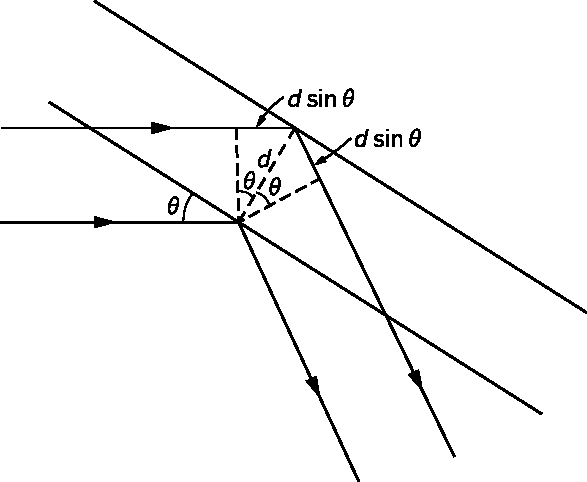
\includegraphics[width=1\linewidth]{fyz_fig435.pdf}
      \caption{Rozptyl vln na krystalových rovinách (\cite[s.~514]{Feynman01})}
      \label{fyz:fig435}
    \end{figure}

    Vezmeme-li dvě rovnoběžné roviny, jako na obr. \ref{fyz:fig435}, vlny, které se od nich
    odrazily, budou ve fázi za předpokladu, že rozdíl vzdáleností, které překonají čela vln, je
    roven celému násobku vlnových délek. Je vidět, že tento rozdíl je \(2d\sinθ\), kde \(d\) je
    kolmá vzdálenost mezi rovinami. Takže podmínkou pro koherentní odraz je, aby 
    \begin{equation}\label{fyz:eq604} 
      2d\sinθ = nλ \qquad(n=1,2,…).
    \end{equation}

    Máme-li například krystal, jehož roviny splňují podmínku (\ref{fyz:eq604}) pro \(n = 1\), bude
    odraz silný. Na druhé straně, jsou-li v polovině vzdáleností mezi rovinami další atomy (se
    stejnou hustotou), tyto intermediální roviny budou také způsobovat stejně silný rozptyl a
    interference způsobí, že výsledný efekt bude nulový. Proto se \(d\) musí vztahovat na přilehlé
    roviny; vztah (\ref{fyz:eq604}) nemůžeme použít pro roviny vzdálené o pět vrstev! 
    
    Pro zajímavost: Krystaly nejsou ve skutečnosti tak, jednoduché, aby se v nich určitým způsobem
    opakoval stejný druh atomů. Kdybychom chtěli provést jejich dvourozměrné analýzy, velmi by se
    podobal tapetě, na níž se pravidelně opakuje nějaký vzor. Vzorem v případě atomů rozumíme nějaké
    jejich seskupení: například pro uhličitan vápenatý atom vápníku, atom uhlíku a tři atomy
    kyslíku - kde může být relativně velký počet atomů. Ať je vzor jakýkoliv, vždy se opakuje. Tento
    základní vzorek se nazývá \emph{jednotkovou buňkou}. 
    
    Různé druhy opakování vzorků definují to, čemu říkáme \textbf{typ mřížky}. Typ mřížky lze poznat
    ihned podle toho, jaké symetrické obrazce vytváří odražené světlo. Podle míst, kde dochází k
    odrazům, určíme typ mřížky, ale abychom zjistili, co je uvnitř každé buňky, musíme vzít v úvahu
    intenzitu rozptylu v různých směrech. Směr, v němž dochází k rozptylu, závisí na druhu mřížky,
    ale jak silný je rozptyl v příslušném směru, je určeno tím, co je v každé jednotkové buňce.
    Tímto způsobem se zjišťuje struktura krystalů. 
    
    \begin{figure}[ht!]
      \centering  
      \subcaptionbox{Kamenná sůl\label{fyz:fig436}}{\luafigure[0.45]{fyz_fig436.jpg}}
      \subcaptionbox{Myoglobin\label{fyz:fig437}}{\luafigure[0.44]{fyz_fig437.jpg}}
      \caption{Fotografie vzorků pomocí rentgenové difrakce (\cite[s.~515]{Feynman01})}
    \end{figure}

    Na Obrázcích \ref{fyz:fig436} a \ref{fyz:fig437} jsou dvě fotografie vzorků pomocí rentgenové
    difrakce. Znázorňují rozptyl na kamenné soli a na myoglobinu (červené barvivo svalu).  
    
    Zajímavá situace nastává, jsou-li sousední krystalové roviny od sebe vzdáleny o méně než
    \(λ/2\). V tom případě podmínka (\ref{fyz:eq604}) nemůže být splněna. Proto je-li \(\lambda\)
    větší než dvojnásobek vzdálenosti mezi sousedními rovinami, nevzniká žádný difrakční vzor a
    světlo (nebo cokoliv) projde materiálem, aniž by se odráželo nebo ztrácelo. Je-li \(\lambda\) v
    případě světla mnohem větší než vzdálenost mezi rovinami, prochází světlo krystalem, aniž by
    docházelo k jeho odrazu od rovin krystalu.  
    
    \begin{figure}[ht!] %\ref{fyz:fig438}
      \centering
      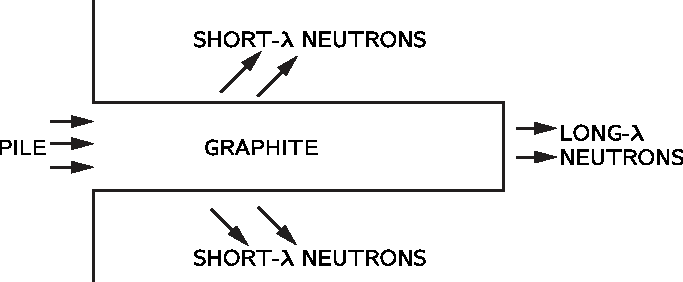
\includegraphics[width=0.9\linewidth]{fyz_fig438.pdf}
      \caption{Difúze neutronů z reaktoru grafitovým blokem (\cite[s.~515]{Feynman01})}
      \label{fyz:fig438}
    \end{figure}

    To má zajímavý důsledek pro neutrony z reaktoru (jsou to zřejmě částice za všechny peníze!).
    Postavíme-li jim do cesty blok z grafitu, neutrony difundují a razí si jím cestu (obr.
    \ref{fyz:fig438}). Difundují, neboť se srážejí s atomy, ale přesně řečeno podle vlnové teorie,
    odrážejí se, neboť dochází k jejich difrakci na krystalových rovinách. Neutrony, jež vylétají z
    velmi velkého kusu grafitu na druhém konci, mají všechny velkou vlnovou délku! Když si graficky
    znázorníme jejich intenzitu jako funkci vlnové délky, vidíme, že je různá od nuly jen pro vlnové
    délky větší než určitá minimální délka (obr. \ref{fyz:fig439}). Znamená to, že tak můžeme získat
    velmi pomalé neutrony. Grafitem proletí jen ty nejpomalejší neutrony, které se na krystalových
    rovinách nedifragují nebo nerozptylují, ale letí přímo skrz jako světlo sklem a nerozptylují se
    do stran. Je mnoho jiných důkazů existence neutronových vln a vln jiných částic.

    \begin{figure}[ht!] %\ref{fyz:fig439}
      \centering
      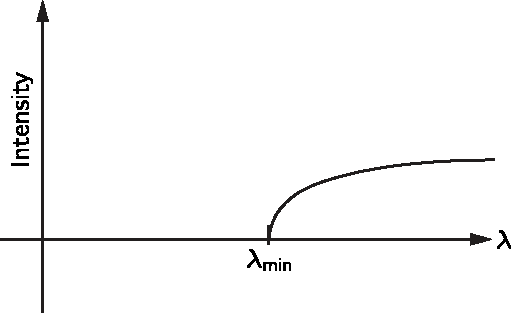
\includegraphics[width=0.8\linewidth]{fyz_fig439.pdf}
      \caption{Intenzita neutronů vyletujících z grafitového bloku jako funkce vlnové délky
              (\cite[s.~516]{Feynman01})}
      \label{fyz:fig439}
    \end{figure}

  \section{Velikost atomu}\label{fyz:IchapXXXVIIIsecIV}
    Nyní se zamyslíme nad jinou aplikací principu neurčitosti vyjádřeného rovnicí (\ref{fyz:eq597}).
    Tuto aplikaci nesmíme brát příliš vážně. Myšlenka je správná, ale naše analýza nebude moc
    přesná. Týká se demonstrace rozměrů atomů a toho, že podle klasické teorie by měly elektrony
    vyzařovat světlo a obíhat po spirále, dokud nespadnou na jádro. To však nemůže být v souladu s
    kvantovou mechanikou, kde nemůžeme vědět, kde byl každý elektron a jak rychle se pohyboval. 

    Představme si, že chceme určit polohu elektronu ve vodíkovém atomu. Je nemožné, abychom přesně
    určili jeho polohu, neboť pak by byla neurčitost jeho hybnosti nekonečná. Kdykoliv se na
    elektron podíváme, někde se nachází; má však určitou amplitudu pravděpodobnosti, vyskytovat se
    na různých místech. Tato místa se nemohou nacházet všechna v jádře; budeme předpokládat, že jsou
    rozložena ve vzdálenosti a od jádra, tj. že vzdálenost elektronu od jádra je obvykle řádově
    rovna \(a\). Minimalizací celkové energie atomu určíme \(a\). 
    
    Ze vztahu neurčitosti vyplývá, že neurčitost hybnosti je \(ℏ/a\), takže kdybychom chtěli nějak
    změřit hybnost elektronu, například pomocí rozptylu rentgenových paprsků na elektronu a
    sledováním Dopplerova jevu na pohybujícím se rozptylovém centru, očekávali bychom, že
    nedostaneme vždy nulu - elektron nebude stát na místě - ale jeho hybnost musí být řádově
    \(p≈ℏ/a\). Kinetická energie je přibližně  \(\frac{1}{2}mv^2=\frac{p^2}{2m}=\frac{ℏ^2}{2ma^2}\).
    (V určitém smyslu provádíme jistý druh rozměrové analýzy, jak závisí kinetická energie na
    Planckově konstantě, na \(m\) a rozměrech atomu. Naší odpovědi můžeme důvěřovat s přesností na
    faktory jako 2, \(\pi\) atd. Dokonce ani \(a\) jsme nedefinovali moc přesně.) Potenciální energie
    je rovna \(e^2\) dělenému vzdáleností od středu, \(-\frac{e^2}{a}\), kde \(e^2\) (jak si
    pamatujeme) je rovna druhé mocnině náboje elektronu dělené \(4\pi\varepsilon_0\). Vtip je nyní v
    tom, že potenciální energie klesá, když se \(a\) zmenšuje, ale čím je menší \(a\), tím je podle
    principu neurčitosti větší hybnost a tedy i kinetická energie. Celková energie je 
    \begin{equation}\label{fyz:eq605}
      E=\frac{ℏ^2}{2ma^2} - \frac{e^2}{a}.
    \end{equation}    
    Nevíme, čemu je rovno \(a\), ale víme, že atom se uspořádá tak, aby došlo k určitému kompromisu
    a aby jeho energie byla tak malá, jak jen může být. Abychom našli minimum \(E\), zderivujeme ji
    podle \(a\), položíme derivaci rovnu nule a z této rovnice najdeme \(a\). Derivace \(E\) je
    rovna 
    \begin{equation}\label{fyz:eq606}
      \der{E}{a}=-\frac{ℏ^2}{ma^3} + \frac{e^2}{a^2},
    \end{equation}    
    a když ji položíme rovnu nule, dostaneme pro hodnotu \(a\) 
    \begin{equation}\label{fyz:eq607}
      a_0=\frac{ℏ^2}{me^2} = \SI{0.528e-10}{\m}.
    \end{equation}    
    Tato vzdálenost se nazývá \textbf{Bohrův poloměr} a tak jsme se dozvěděli, že rozměry atomů jsou
    řádově \SI{10e-10}{\m} , což je pravda. To je krásné - je to úžasné, neboť do této doby jsme
    neměli žádnou bázi, na jejímž základě bychom mohli odhadnout rozměry atomů! Přitom z klasického
    hlediska atomy vlastně nemohou existovat, neboť elektrony by měly spadnout po spirále na jádro. 
    
    Dosadíme-li hodnotu pro \(a_0\) z (\ref{fyz:eq607}) do vztahu pro energii (\ref{fyz:eq605}),
    dostáváme 
    \begin{equation}\label{fyz:eq608}
      E_0 = −\frac{e^2}{2a_0} = −\frac{me^4}{2ℏ^2} = \SI{-13.6}{\eV}.
    \end{equation}
    
    Co znamená záporná energie? Znamená, že elektron má v atomu menší energii, než když je volný.
    Znamená to, že je vázaný. Znamená to, že k uvolnění elektronu je třeba energie. K ionizaci
    vodíkového atomu musíme dodat energii \SI{13.6}{\eV}. Nemáme důvod, abychom si nemysleli, že má
    být dvakrát nebo třikrát větší než tato energie - nebo poloviční nebo \(1/\pi\) násobek, když
    naše argumentace byla taková ledabylá. My jsme však trochu podváděli, použili jsme takové
    konstanty, aby nám vyšlo správné číslo! Hodnota \num{13.6} elektronvoltů se nazývá
    \textbf{Rydbergova energie}. Je to ionizační energie vodíkového atomu. 
    
    Ted' alespoň chápeme, proč se nepropadneme podlahou. Když jdeme, naše boty tlačí svými atomy na
    atomy podlahy. Kdybychom stlačili atomy blíže k sobě, musely by elektrony zabírat menší prostor
    a podle principu neurčitosti by se musely v průměru zvýšit jejich hybnosti, což by znamenalo
    vyšší energii. Odpor při stlačování atomů je kvantově-mechanický efekt a ne klasický efekt.
    Klasicky bychom předpokládali, že kdybychom k sobě přiblížili všechny elektrony a protony,
    energie by se stále zmenšovala. Nejvýhodnější seskupení kladných a záporných atomů v klasické
    fyzice je, když jsou všechny těsně u sebe. V klasické fyzice to bylo dobře známé a existence
    atomů byla záhadou. Samozřejmě, vědci tehdy objevili několik způsobů, jak se dostat z těžkostí,
    ale teprve my jsme našli ten správný způsob! (Snad.) 
    
    I když nemáme předpoklady, abychom tomu na naší úrovni porozuměli, zmíníme se o tom, že tam, kde
    je mnoho elektronů, snaží se být od sebe co nejdále. Obsadí-li jeden elektron určitý prostor,
    druhý elektron ho neobsadí. Přesněji řečeno existují dva případy spinu, takže dva elektrony
    mohou ještě „sedět“ jeden na druhém, přičemž mají opačné spiny, ale víc jich tam už nemůžeme
    dát. Ostatní musíme dát na jiná místa, a to je skutečný důvod, proč má hmota pevnost. Když
    bychom mohli umístit všechny elektrony na stejné místo, hmota by se zkondenzovala ještě víc než
    nyní. Právě této skutečnosti, že všechny elektrony se nemohou shluknout v jednom místě, vděčíme
    za to, že stoly a jiné věci jsou pevné. 
    
    K pochopení vlastností hmoty budeme muset zřejmě použít kvantovou mechaniku a nemůžeme se
    spokojit s klasickou mechanikou.
  
  \section{Energetické hladiny}\label{fyz:IchapXXXVIIIsecV}
    Mluvili jsme o atomu v nejnižším možném energetickém stavu, ale jak je vidět, elektron dokáže i
    jiné věci. Může se vrtět a kmitat mnohem energičtěji, takže v atomu existuje mnoho různých
    pohybů. Podle kvantové mechaniky může mít atom určitou energii jen ve stacionárním stavu. Na
    obrázku \ref{fyz:fig440} máme diagram, kde nanášíme energii na svislou osu a pro každou
    dovolenou energii máme nakreslenou vodorovnou čáru. Je-li elektron volný, tj. je-li jeho energie
    kladná, jeho energie může být libovolná, může se tedy pohybovat libovolnou rychlostí. Energie
    vázaného elektronu však nejsou libovolné. Atomy musí mít některou z dovolených hodnot energie,
    jako jsou ty na obr. \ref{fyz:fig440}.
    \begin{figure}[ht!] %\ref{fyz:fig440}
      \centering
      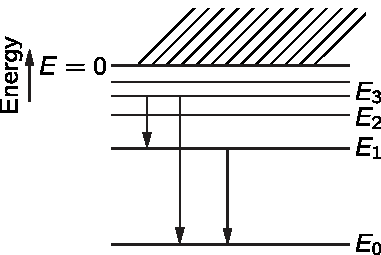
\includegraphics[width=0.7\linewidth]{fyz_fig440.pdf}
      \caption{Energetické schéma atomu znázorňující několik možných přechodů
              (\cite[s.~518]{Feynman01})}
      \label{fyz:fig440}
    \end{figure}

    Označme dovolené hladiny energie \(E_0\), \(E_l\), \(E_2\), \(E_3\). Nachází-li se atom v
    některém z excitovaných vzbuzených stavů \(E_l\), \(E_2\) atd., nezůstane v něm navždy. Dříve
    nebo později klesne do nižšího stavu a vyzáří energii ve formě světla. Frekvencí emitovaného
    světla lze určit pomocí zákona zachování energie a kvantově-mechanického chápání toho, že
    frekvence světla souvisí s jeho energií podle (\ref{fyz:eq598}). Proto frekvence světla, jež se
    uvolní při přechodu od energie \(E_3\) k energii \(E_l\) (například), je
    \begin{equation}\label{fyz:eq609}
      ω_{31} = \frac{(E_3−E_1)}{ℏ}.
    \end{equation}
    To je pak charakteristická frekvence atomu a definuje jeho spektrální emisní čáru. Další možný
    přechod by byl od \(E_3\) k \(E_0\). Ten bude odpovídat frekvenci
    \begin{equation}\label{fyz:eq610}
      ω_{30} = \frac{(E_3−E_0)}{ℏ}.
    \end{equation}
    Další možnost je ta, že když byl atom vzbuzen do stavu \(E_1\), může spadnout do základního
    stavu \(E_0\), přičemž vyzáří foton s frekvencí
    \begin{equation}\label{fyz:eq611}
      ω_{10} = \frac{(E_1−E_0)}{ℏ}.
    \end{equation}
    Tyto tři přechody jsme vybrali proto, abychom mohli ukázat na zajímavý vztah. Z
    (\ref{fyz:eq609}), (\ref{fyz:eq610}) a (\ref{fyz:eq611}) je snadno vidět, Že
    \begin{equation}\label{fyz:eq612}
      ω_{30} = ω_{31} + ω_{10}.
    \end{equation}

    Obecně platí, že najdeme-li dvě spektrální čáry, můžeme očekávat, že další najdeme na součtu
    jejich frekvencí (nebo na rozdílu jejich frekvencí). Tyto čáry můžeme objasnit pomocí série
    hladin tak, že každá čára odpovídá rozdílu energií nějakého páru energetických hladin. Tato
    pozoruhodná shoda spektrálních frekvencí byla objevena dříve, než kvantová mechanika a nazývá se
    \textbf{Ritzův kombinační princip}. Z hlediska klasické mechaniky je to opět záhada. Nemusíme se
    dále snažit zdůrazňovat, že klasická fyzika selhává v oblasti atomů, zdá se, že jsme to dokázali
    dostatečně jasně.

    Již jsme si řekli, že kvantová mechanika je reprezentována pomocí amplitud, jež se chovají jako
    vlny s určitými frekvencemi a vlnovými čísly. Podívejme se, jak plyne z hlediska amplitud, že
    atom má určité energetické stavy. Je to něco, co nemůžeme pochopit z toho, co jsme si dosud
    řekli, ale všichni víme, že stojaté vlny mají určité frekvence. Například zvuk uzavřený ve
    varhanní píšťale však může vibrovat více způsoby, přičemž každému z nich přísluší určitá
    frekvence. Proto má objekt, v němž jsou vlny uzavřené, určité rezonanční frekvence. To, že
    vlnění může existovat jen při určitých frekvencích, je vlastnost vln v uzavřeném prostoru. O tom
    budeme mluvit podrobně včetně vzorců až později. A protože mezi frekvencemi amplitud a energií
    existuje obecný vztah, nejsme překvapení, že s elektrony vázanými v atomech souvisí jen určité
    energie.

  \section{Filozofické důsledky}\label{fyz:IchapXXXVIIIsecVI}
    Proberme si stručně některé filozofické důsledky vyplývající z kvantové mechaniky. Jako vždy má
    tento problém dvě stránky: jednou jsou filozofické důsledky pro fyziku a druhou jejich extrapolace
    do jiných oblastí. Když se filozofické myšlenky, spojené s přírodní vědou, přenášejí do jiných
    oblastí, obvykle se zcela překroutí. Proto naše poznámky omezíme, pokud to bude možné, jen na
    fyziku. 
    
    Nejzajímavějším aspektem je především myšlenka principu neurčitosti; pozorování nějakého jevu
    ovlivňuje samotný jev. Vždy bylo známo, že pozorováním nějakého jevu se tento jev ovlivňuje, ale
    jde tady o to, že toto ovlivňování nelze zanedbat, minimalizovat nebo libovolně zmenšovat pomocí
    vhodného uspořádání aparatury. Sledujeme-li nějaký jev, nemůžeme si pomoci, ale musíme ho aspoň
    minimálním způsobem narušit \emph{a toto narušení je nevyhnutné pro konzistentnost našeho
    chápání}. V předkvantové fyzice byl někdy pozorovatel důležitý, ale jen v triviálním smyslu. Byl
    nastolen takový problém: Když v lese padne strom a není tam nikdo, kdo by to slyšel, vzniká
    přitom zvuk? Přirozeně, pádem skutečného stromu ve skutečném lese vzniká zvuk, i kdyby tam nikdo
    nebyl. I když tam nikdo není, kdo by to slyšel, zůstanou i jiné stopy. Zvuk rozechvěje listy a
    kdybychom byli dostatečně pozorní, snad bychom zjistili, že se někde nějaký trn otřel o list a
    jemně ho poškrábal, což nelze vysvětlit bez předpokladu, že se list rozechvěl. Takže v určitém
    smyslu musíme přiznat, že při tom vzniká zvuk. Můžeme se zeptat: Došlo přitom k pocitu zvuku?
    Ne, pociťování zřejmě Souvisí s vědomím. A zda si to uvědomili mravenci, zda byli nějací
    mravenci v lese nebo zda si to uvědomil strom, to nevíme. Nechme tento problém tak, jak je. 
    
    Další věc, kterou lidé zdůrazňovali před kvantovou mechanikou, je myšlenka, že bychom neměli
    mluvit o věcech, jež nemůžeme měřit. (Skutečně to tvrdila i teorie relativity.) Nemůžeme-li něco
    určit měřením, nemá to v teorii co hledat. Protože přesnou hodnotu hybnosti lokalizované částice
    nelze měřením určit, nemá v teorii místo. Představa, že tak to bylo v klasické teorii, je
    falešná. je důsledkem nedbalé analýzy situace. Nemožnost přesného měření polohy a hybnosti ještě
    \emph{a priori} neznamená, že o nich nemůžeme mluvit. Znamená to jen tolik, že o nich nemusíme
    mluvit. Ve vědě je taková situace: Pojem nebo představa, kterou nelze měřit nebo nelze přímo
    odvodit z experimentu, může být, ale nemusí být užitečná. Nemusí existovat v teorii. jinými
    slovy, předpokládejme, že porovnáme klasickou teorii světa s kvantovou teorií a předpokládejme,
    že experimentálně platí fakt, že jak polohu, tak i hybnost můžeme měřit jen nepřesně. Vzniká
    otázka, zda představa přesné polohy částice a představa přesné hybnosti částice platí nebo ne.
    Klasická teorie tyto představy připouští, kvantová teorie nepřipouští. To samo o sobě ještě
    neznamená, že klasická fyzika je chybná. Když byla objevena kvantová mechanika, klasici (to byli
    všichni kromě Heisenberga, Schrödingera a Borna) říkali: „Podívejte se, vaše teorie nestojí za
    nic, protože neumíte dát odpovědi na určité otázky jako například: jaká je přesná poloha
    částice? Kterým otvorem prošla? atd.“ Heisenbergova odpověď' zněla: „Nepotřebujeme odpovědi na
    tyto otázky, protože vy je nemůžete experimentálně ověřit.“ Vtip je v tom, že nemusíme. Vezměme
    si dvě teorie: \(a\) a \(b\). Teorie a obsahuje představu, kterou nelze přímo ověřit, ale která
    se používá při analýze a teorie b tuto představu neobsahuje. Když se teorie ve svých
    předpovědích neshodnou, nelze tvrdit, že b je špatná, protože neumí vysvětlit představu, kterou
    používá a, neboť je to představa, jež patří mezi ty, co nelze přímo ověřit. je vždy dobré, když
    víme, které představy nelze přímo ověřit, ale ne vždy je nutné je všechny odstranit. Není
    pravda, že vědu můžeme posunout dále jen pomocí koncepcí, jež přímo souvisí s experimentem. 
    
    Kvantová mechanika obsahuje amplitudu vlnové funkce, potenciál a mnoho dalších konstrukcí, jež
    nelze přímo měřit. Podstata vědy spočívá v její schopnosti \emph{předpovídat}. Předpovídat
    znamená říci, co se stane v experimentu, který ještě nikdo nikdy neudělal, jak to můžeme vědět?
    Nezávisle na experimentu předpokládáme, že víme, co při něm probíhá. Musíme extrapolovat
    experimenty do oblasti, kde se ještě nedělaly. Musíme své představy rozšířit na situace, v nichž
    je ještě nikdo neprověřil. Když to neuděláme, nemáme předpověď'. Proto se klasickým fyzikům
    zdálo rozumné předpokládat, že poloha – jež má jasný smysl v bejsbolu – bude mít smysl i pro
    elektron. Nebyl to projev hlouposti. Byl to rozumný proces. Dnes říkáme, že Zákon relativity
    platí pro všechny energie, ale jednou může někdo přijít a říci, jací jsme byli hloupí. V čem
    jsme „hloupí“, nevíme, dokud „nevystrčíme hlavu ven“. Celá idea spočívá v tom, abychom vystrčili
    ven hlavu. jediný způsob, jak můžeme zjistit, že se mýlíme, je ten, že se podíváme, jaké jsou
    naše předpovědi je nutné, abychom vymýšleli nové konstrukce. Už jsme udělali několik poznámek o
    neurčitosti kvantové mechaniky. O tom, že nejsme schopni předpovědět, co se fyzikálně stane za
    daných fyzikálních podmínek, jež jsou uspořádány tak pečlivě, jak jen lze. Máme-li atom, který
    je v excitovaném stavu a který se chystá vyzářit foton, nemůžeme říci, kdy ho vyzáří. V každém
    okamžiku má určitou amplitudu, že foton vyzáří a my umíme předpovědět jen pravděpodobnost emise;
    nemůžeme předpovědět budoucnost přesně. To dalo podnět ke vzniku všelijakých nesmyslů, k otázkám
    o smyslu svobodné vůle a k myšlence, že svět je neurčitý. 
    
    Musíme zdůraznit, že klasická fyzika je také v určitém smyslu indeterministická. Obyčejně se má
    za to, že tato vlastnost, tj. že nemůžeme předpovědět budoucnost, je důležitá kvantové –
    mechanická vlastnost a tím by se mělo vysvětlovat myšlení, city, vůle atd. Kdyby svět byl
    klasický – kdyby byly jen klasické zákony mechaniky – není vůbec zřejmé, že mysl by nepracovala
    více méně stejně. je pravda, že kdybychom klasicky znali polohu a rychlost každé částice ve
    světě nebo v krabici s plynem, mohli bychom exaktně předpovědět, co bude. Proto je klasický svět
    deterministický. Předpokládejme však, že máme konečnou přesnost a že známe polohu každého atomu
    dejme tomu s přesností jedné miliardtiny. Pak tento atom narazí do dalšího atomu a když jsme
    jeho polohu neznali přesněji než na jednu miliardtinu, bude po srážce nepřesnost v jeho poloze
    ještě větší. Další srážkou se chyba ještě zvětší, takže, když začneme třeba jen s malými
    chybami, ty rychle narostou na velmi velkou neurčitost. Uvedeme příklad. Voda se při pádu z
    přehrady tříští a stojíme-li někde blízko, tu a tam nám na nose přistane kapka. Zdá se to být
    zcela náhodné, a přece by se to dalo předpovědět pomocí klasických zákonů. Přesné polohy kapek
    závisí na proudění vody dřív, než protéká přes přehradu. Jak? Nejmenší nahodilosti se ve
    vodopádu zesilují, takže dostáváme úplnou nahodilost. Je jasné, že polohy kapek nemůžeme reálně
    předpovědět, když neznáme pohyb vody \emph{naprosto přesně}. 
    
    Přesněji řečeno, při libovolné přesnosti lze najít dostatečně vzdálený čas, pro který nemůžeme
    udělat platné předpovědi. Vtip je v tom, že tento čas není ani příliš vzdálený. Věc se nemá tak,
    že by přesnosti na jednu miliardtinu odpovídal čas miliónů roků. Čas se fakticky mění jen
    logaritmicky ve srovnání s chybou a ukazuje se, že už za velmi krátký čas ztrácíme celou
    informaci. Je-li přesnost dána na jednu miliardtinu z miliardtiny (můžeme vzít miliardtin kolik
    chceme, jen když se někde zastavíme), zjistíme, že čas, po němž už nemůžeme předpovědět, co se
    Stane, je kratší, než byl čas, Za který jsme si stanovili původní přesnost! Není proto čestné
    říkat, že na základě zdánlivé svobody a indeterminizmu lidské myslí jsme si měli uvědomit, že
    klasická „deterministická“ fyzika si nikdy nemohla dělat naději, že to pochopí a vítat kvantovou
    mechaniku jako osvobození od „úplně mechanistického“ vesmíru, neboť z praktického hlediska už
    existoval indeterminizmus v klasické mechanice.
  
  \section{Příklady a cvičení}\label{fyz:IchapXXXVIIIsecVII}
%~~~~~~~~~~~~~~~~~~~~~~~~~~~~~~~~~~~~~~~~~~~~~~~~~~~~~~~~~~~~~~~~~~~~~~~~~~~~~~~~~~~~~~~~~~~~~~~~~~